\documentclass[letterpaper]{article}
\usepackage[letterpaper, left=0.625in, right=0.625in, bottom=1in, top=0.75in]{geometry}
\usepackage{cmap}
\usepackage{multicol}
\usepackage{float}
\usepackage{graphicx}
\usepackage[T1]{fontenc}
\usepackage{lmodern}
\usepackage{amsmath}

\title{Internship report}
\author{Nathan Boyer}

\begin{document}

\maketitle


    


\begin{abstract}
    
    It's possible to distribute the Internet to users via drones.
    However, this raises the question of how to place the drones around the users, and how to distribute the bandwidth between the different users.
    A reinforcement AI has already been designed to address this problem.
    However, in this article, we will see how learning and optimization can be combined to further improve performance.

\end{abstract}


\section{Probleme presentation}

We have m users, classified into 3 categories, each class having its own bandwidth demand for a drone.
We then want to place n drones, and for each drone, decide how much of its bandwidth it gives to each class of drone, so that as many drones as possible are satisfied, i.e.\:the bandwidth available to them is greater than or equal to their demand.

\section{Problem solving by constrained optimization}

\subsection{In-depth explanation}

This problem can be solved by constrained optimization.

First, we have to define the equation that computes how well a user will reveive a base station's connection depending on where it is.

We have the following Equations for the drones's SINRs, which is a factor that represents how much data is effectively receiveed by the user, in relation to the data sent by the base station to the user:

$\operatorname{SINR}_{i, j}^t=\frac{p c \mu\left(y_j, u_i^t\right)\left(\left(\left\|y_j-u_i^t\right\|\right)^2+\left(h\right)^2\right)^{-\alpha / 2}}{\sum\limits_{k \in \mathcal{U} \backslash i} p c \mu\left(y_j, u_k^t\right)\left(\left(\left\|y_j-u_k^t\right\|\right)^2+\left(h\right)^2\right)^{-\alpha / 2}+\sigma^2}$

To evaluate a configuration we will thus proceed as follows:

You first need to associate each user with its nearest base station.

You then share the bandwidth of a base station dedicated to a given class between all users of this class associated to this base station.

Then, you compute each user SINR and decide for the user is satisfied or not.

The percentage of satisfied user is thus what you want to maximize.

\subsection{Optimization problem}

This problem can be resolved by as an optimization problem, I will show you how to resolve it for 2 base stations.

Let's first define u a matrix of dimensions $N*N$, with N being the number of positions possible for a base station.
$u_{i,j}$ is a binary variable that is equal to one if and only if the first base station is in position i and the second is position j.

$bw$ is a $3*2$ matrix that represents the bandwidth each base station allocates to each user class.

$\delta$ is a vector that represents for every whether it is satisfied or not.

The function to optimize is then: $\max_{u,bw}\sum_{g\in\mathcal{G}}\delta_g$

Under the following constraints:

\begin{enumerate}
    \item $\sum_{b \in |\mathcal{U}|} \sum_{i, j \in \mathcal{U}} u_{i, j} \times bw_{\text{slice}(g), b} \times \text{bps}_g \frac{100}{G_{\text{conn}}(\text{slice}(g),b)} \nonumber$
    $\geq th_g \times \delta_g \hspace{1cm} \forall g \in \mathcal{G} \\[1em]$
    \item $bw_{em,b} + bw_{ur,b} + bw_{mm,b} = 1 \hspace{1cm} \forall b \in |\mathcal{U}| \\[1em]$
    \item $bw_{em,b} \geq 0; bw_{ur,b} \geq 0; bw_{mm,b} \geq 0 \hspace{1cm} \forall b \in |\mathcal{U}| \\[1em]$
    \item $\sum_{i,j \in \mathcal{U}}u_{i,j} = 1 \\[1em]$
    \item $\delta_g \in \{0, 1\} \hspace{1cm} \forall g \in \mathcal{G} \\[1em] $
    \item $u_{i,j} \in \{0, 1\} \hspace{1cm} \forall i,j \in \{0, 1, \ldots , |\mathcal{U}-1|\}$
\end{enumerate}

The resolution of this optimization problem can be implemented in Python with the help of a module such as pulp.

\subsection{Time Optimizations}

To speed up the resolution of this problem, I implemented a few optimizations:

First, only positions in the convex enveloppe of the users can actually be candidates for optimal placements of the base stations.
We can thus reduce by a lot the size of the matrix u.

Moreover, it is possible to go further but not without losing precision.
Indeed, you can divide the users into k clusters and take the union of this convex enveloppe of this clusters.

You can visualize the transformation done as follows:

\begin{figure}[H]
    \centering
    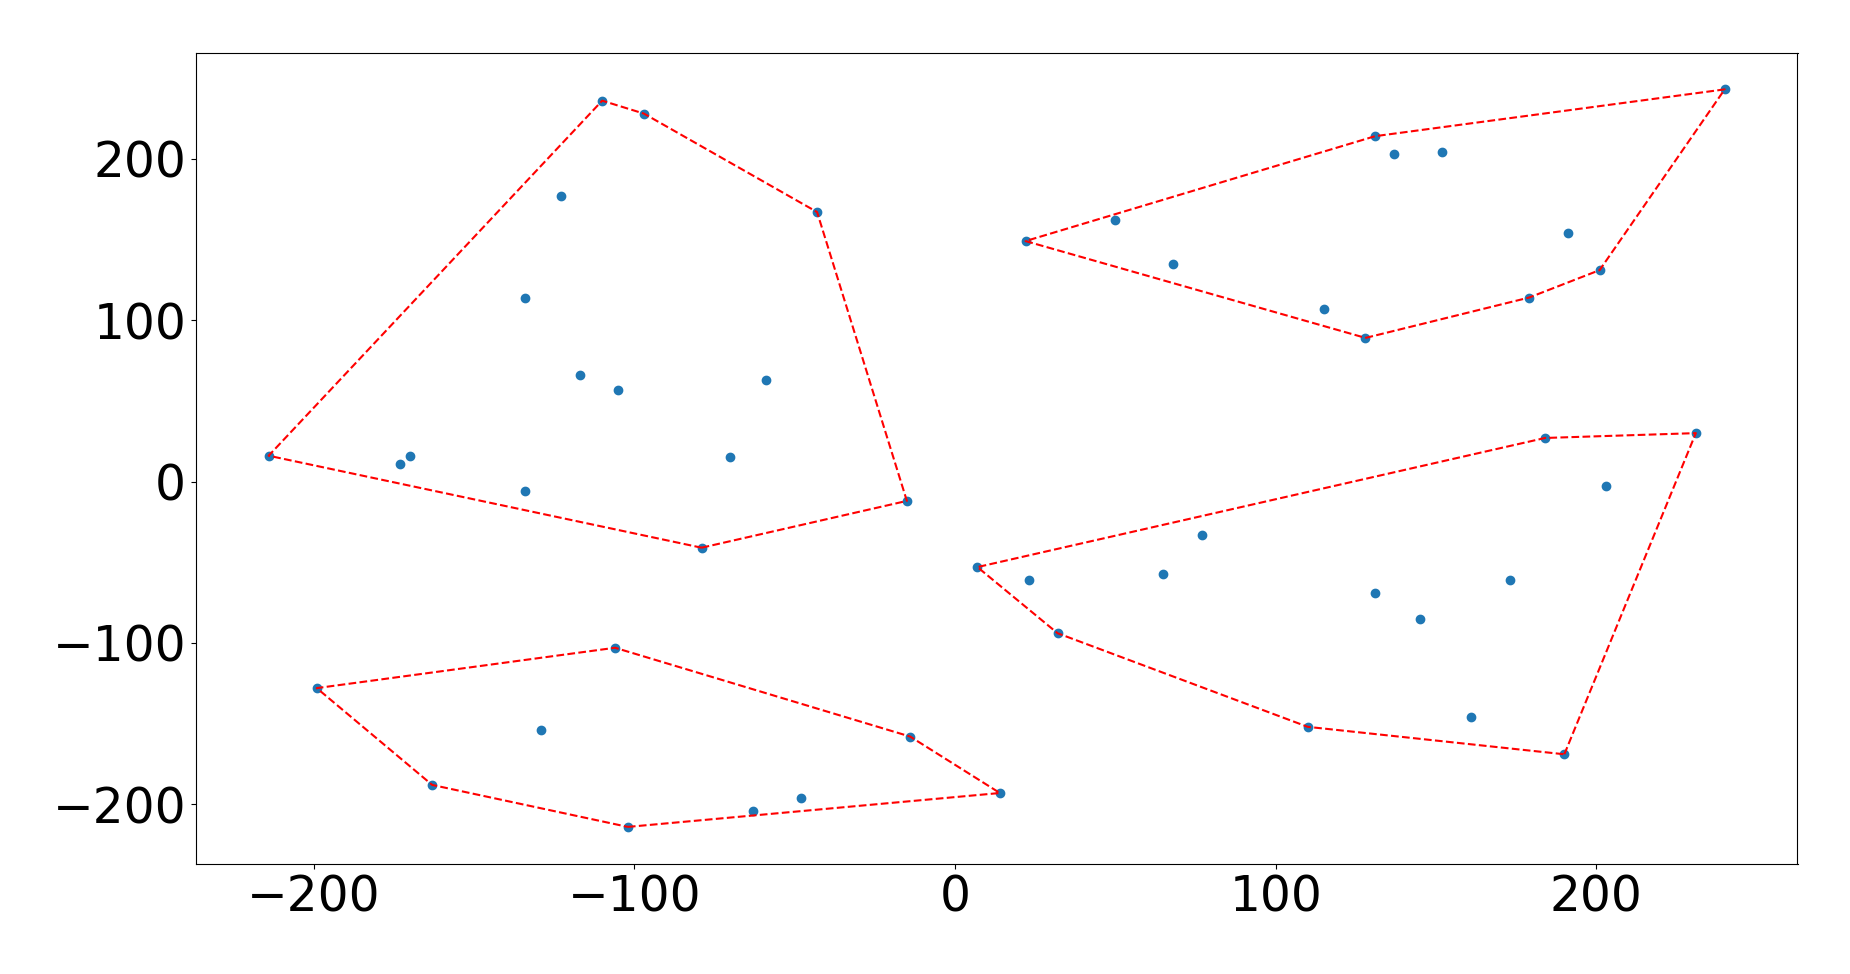
\includegraphics[width=0.5\textwidth]{images/four_cluster.png}
    \caption{Representation of the convex enveloppe of the 4 clusters}
\end{figure}

The graph of performance and time in function of the number of clusters can be found below.

Moreover, I am using \textit{Quote article here} to generate instances, thus as the instances generated have as many
clusters as they have base stations, I am going to generate instances using clusters too.
The performances are then as follows:

\begin{figure}[H]
    \centering
    \begin{minipage}[b]{0.45\textwidth}
        \centering
        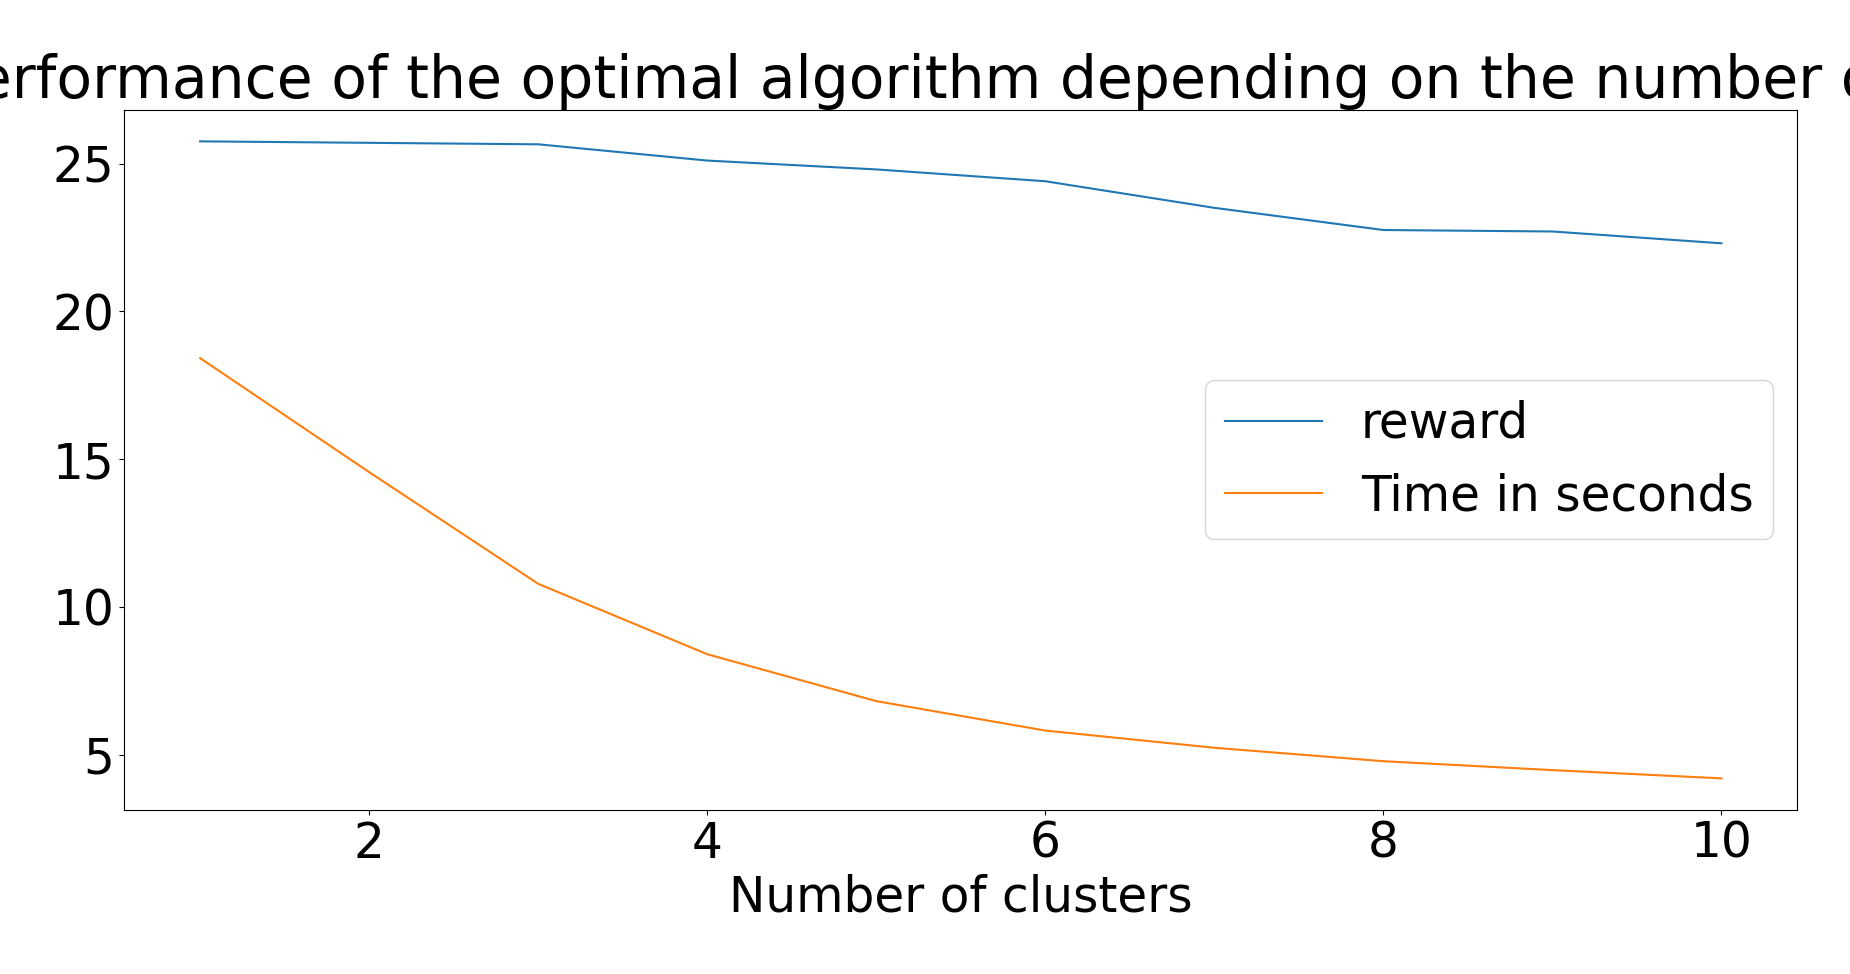
\includegraphics[width=\textwidth]{images/Performance_opt_function_clusters.png}
        \caption{Performance when users are random}
    \end{minipage}
    \hspace{0.05\textwidth}
    \begin{minipage}[b]{0.45\textwidth}
        \centering
        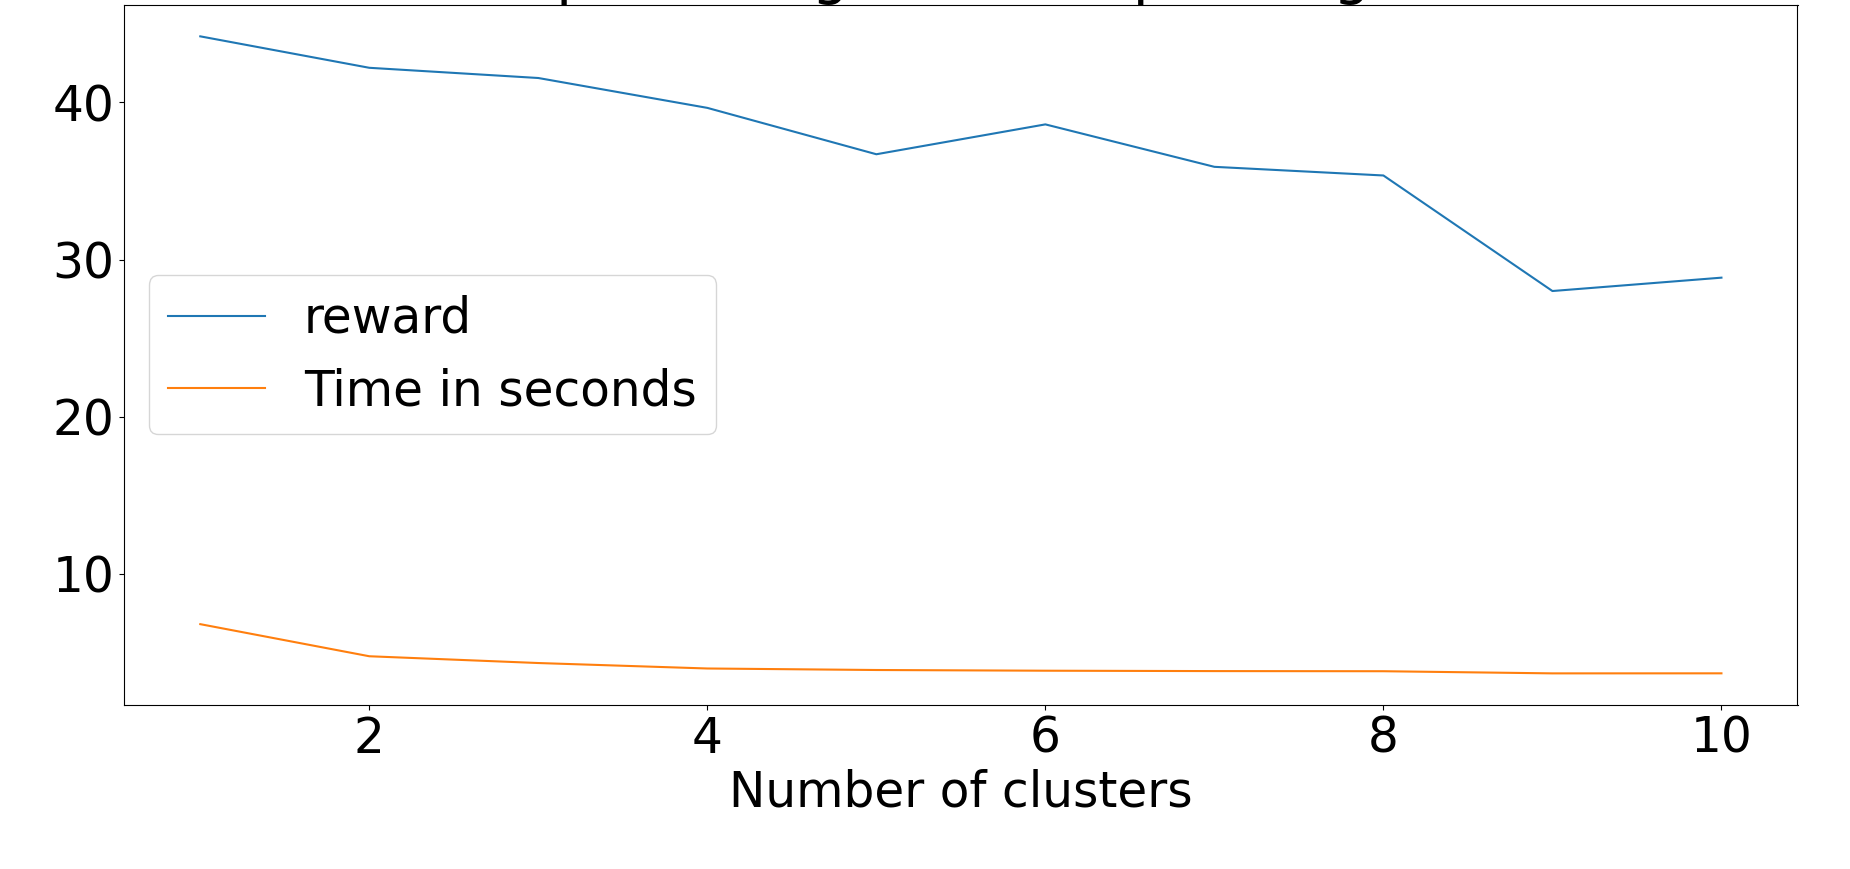
\includegraphics[width=\textwidth]{images/Performance_opt_function_clusters_when_2clusters.png}
        \caption{Performance when users are in 2 clusters}
    \end{minipage}
\end{figure}

However, since the computation times are pretty reasonable for 2 base stations, I decided to go with only 1 cluster.

Finally, multithreading can be used to further accelerate the computations.

\section{Machine learning to solve the problem}

However, a major issue is that this method of solving the problem by optimization is still pretty long.
This can be problematic, especially if the users are moving, and it thus becomes necessary to recalculate the optimal position often.

Thus, a solution using machine learning was considered.
Indeed, solving an instance of the problem would only require a forward pass of the neural network, which is negligible in time.

\subsection{Reinforcement learning}

This is why a reinforcement learning solution was imagined and implemented by Lorenzo Bellone.\textit{Quote article}

He tried to solve the same problem as the one I presented and, to put it shortly, managed to get an average reward of 72-73\% of users satisfied.

However, there are multiple differences between how he approached this problem and how I did:

\begin{enumerate}
    \item First, he moves the base stations setp by step and computes the mean reward over 100 movements.
          However, since the base stations spend most of their times idling (because they have already reached their best possible position),
          I took the bias of putting the base stations directly at the computed best position, and then computing the reward only once (which also allows to test the different agents over more instances in the same amount of time).
    \item Secondly, what is plotted in his article is the average reward during the reinforcement process.
          What it means is that the neural network is only tested on the instances it just learnt from.
          What I did instead is I have a separate test set, which I use to evaluate the different agents.
\end{enumerate}

\subsection{Supervised learning from the optimal solution}

But, an other idea is to use supervised learning.
By using an optimal agent, the neural network can learn to replicate the optimal solutions.

The neural network is then divided in 2 neural networks:

\begin{enumerate}
    \item A neural network that takes as inputs the positions of the users and learns to output the best positions for the 2 base stations.
    \item A neural network that takes as inputs the positions of the users and the positions of the base stations and learns to output the best slicing of bandwiths between the 3 classes of users.
\end{enumerate}

As a side note, the type of each users is represented by 3 one-hots, one for each of the class.

To conclude with my results, here is the average error for the neural network that learns to output the positions:
As well as the average error for the neural network that learns to output the bandwiths:

\begin{figure}[H]
    \centering
    \begin{minipage}[b]{0.45\textwidth}
        \centering
        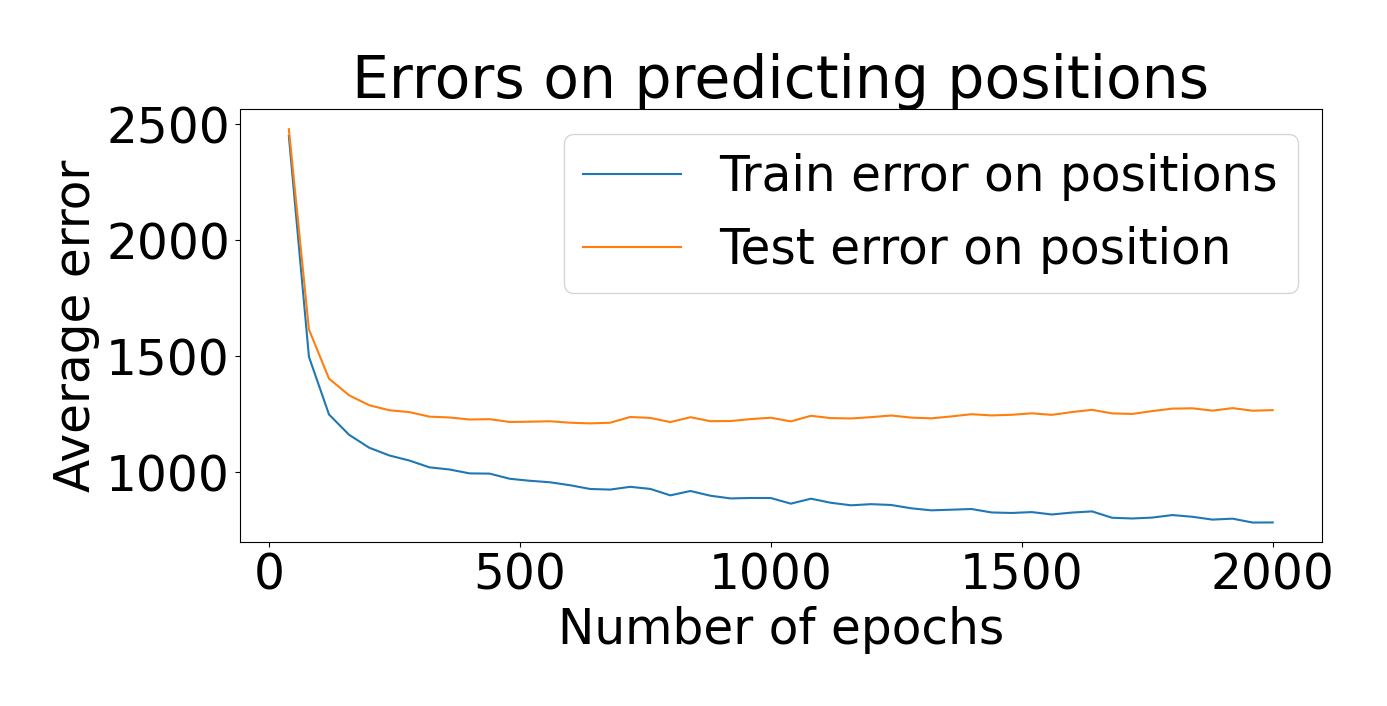
\includegraphics[width=\textwidth]{images/mix_pos.png}
        \caption{Position error}
        \label{fig:image5}
    \end{minipage}
    \hspace{0.05\textwidth}
    \begin{minipage}[b]{0.45\textwidth}
        \centering
        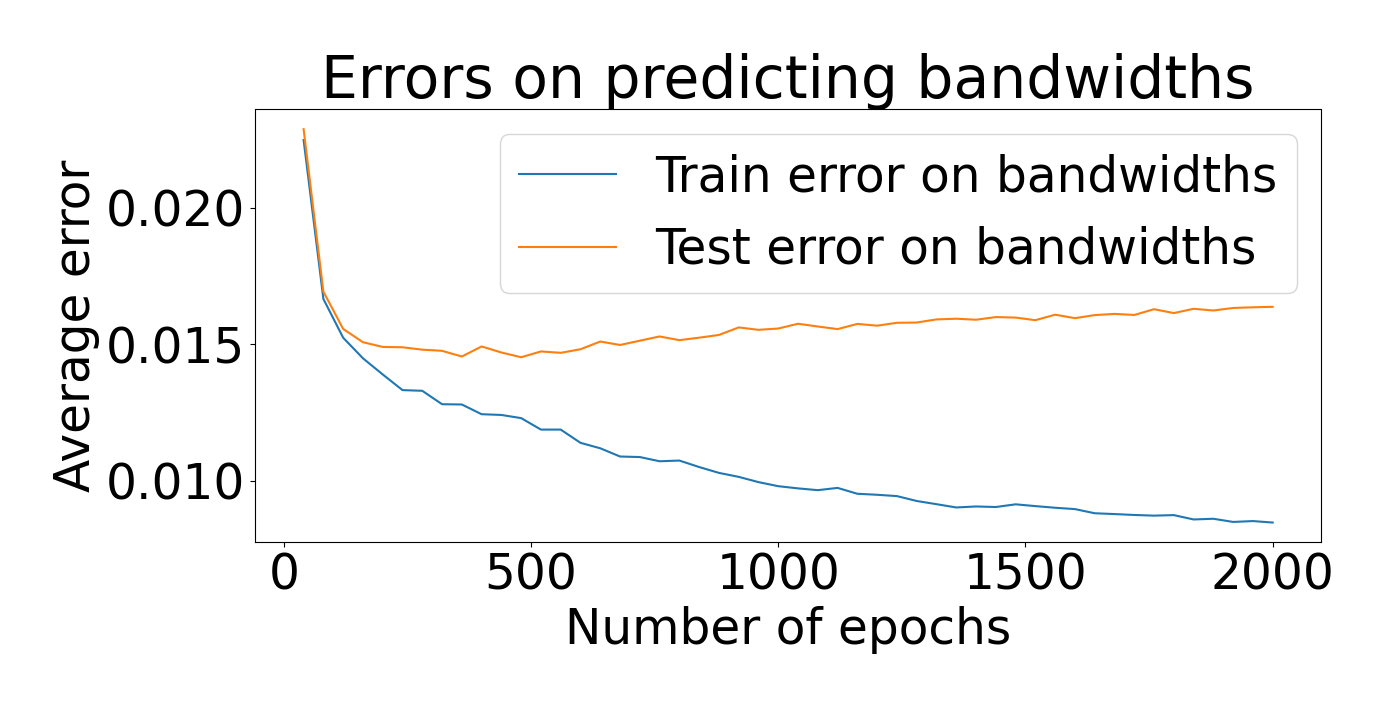
\includegraphics[width=\textwidth]{images/bw_error_epochs.png}
        \caption{Bandwidth error}
        \label{fig:image6}
    \end{minipage}
\end{figure}

\;

With these neural networks, we can test it on instances and evaluate the performances it gives.

(We plot here the normalized average user coverage, i.e.\, the average user coverage divided by the average user coverage of the optimal solution)


\begin{figure}[H]
    \centering
    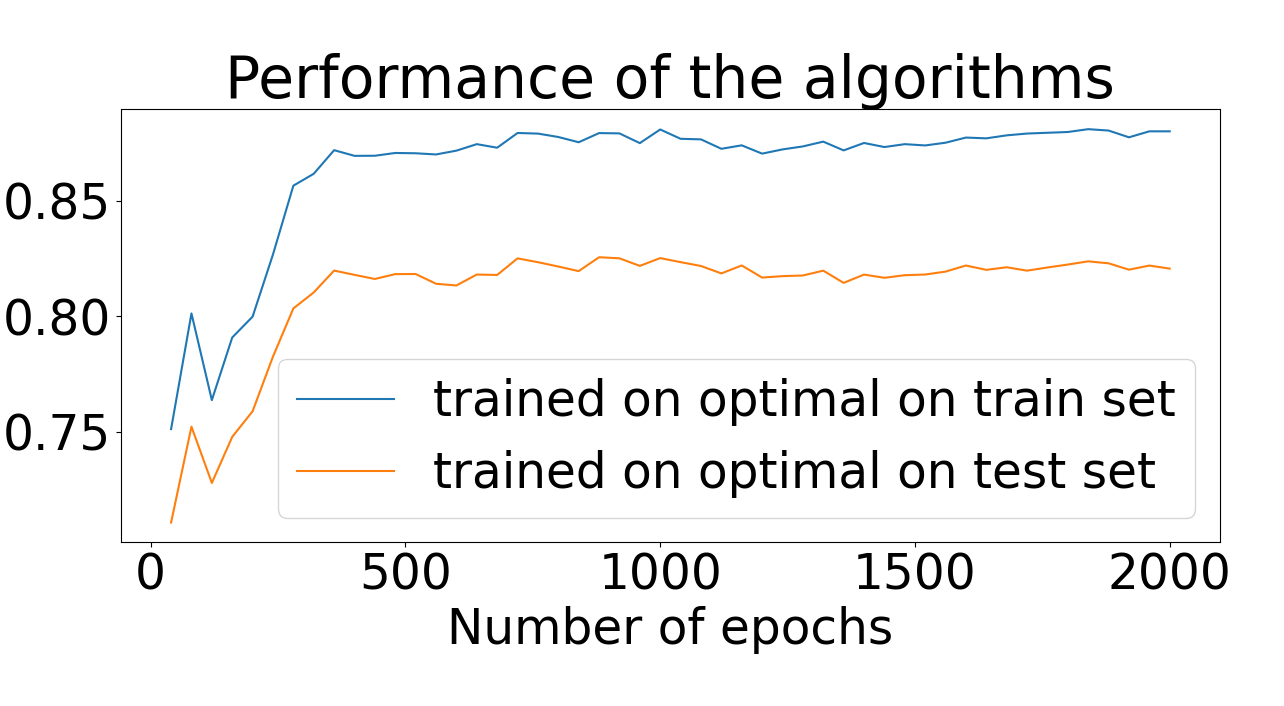
\includegraphics[width=0.5\textwidth]{images/bilan_en _fonction epochs.png}
    \caption{Representation of the convex enveloppe of the 4 clusters}
\end{figure}

\subsection{Learn only what's necessary}

However, you can see the test error on bandwiths stops to decrease rapidly.
That's why I decided to plot the performances when the positions are decided optimally, but the bandwiths are decided with the AI.

\begin{figure}[H]
    \centering
    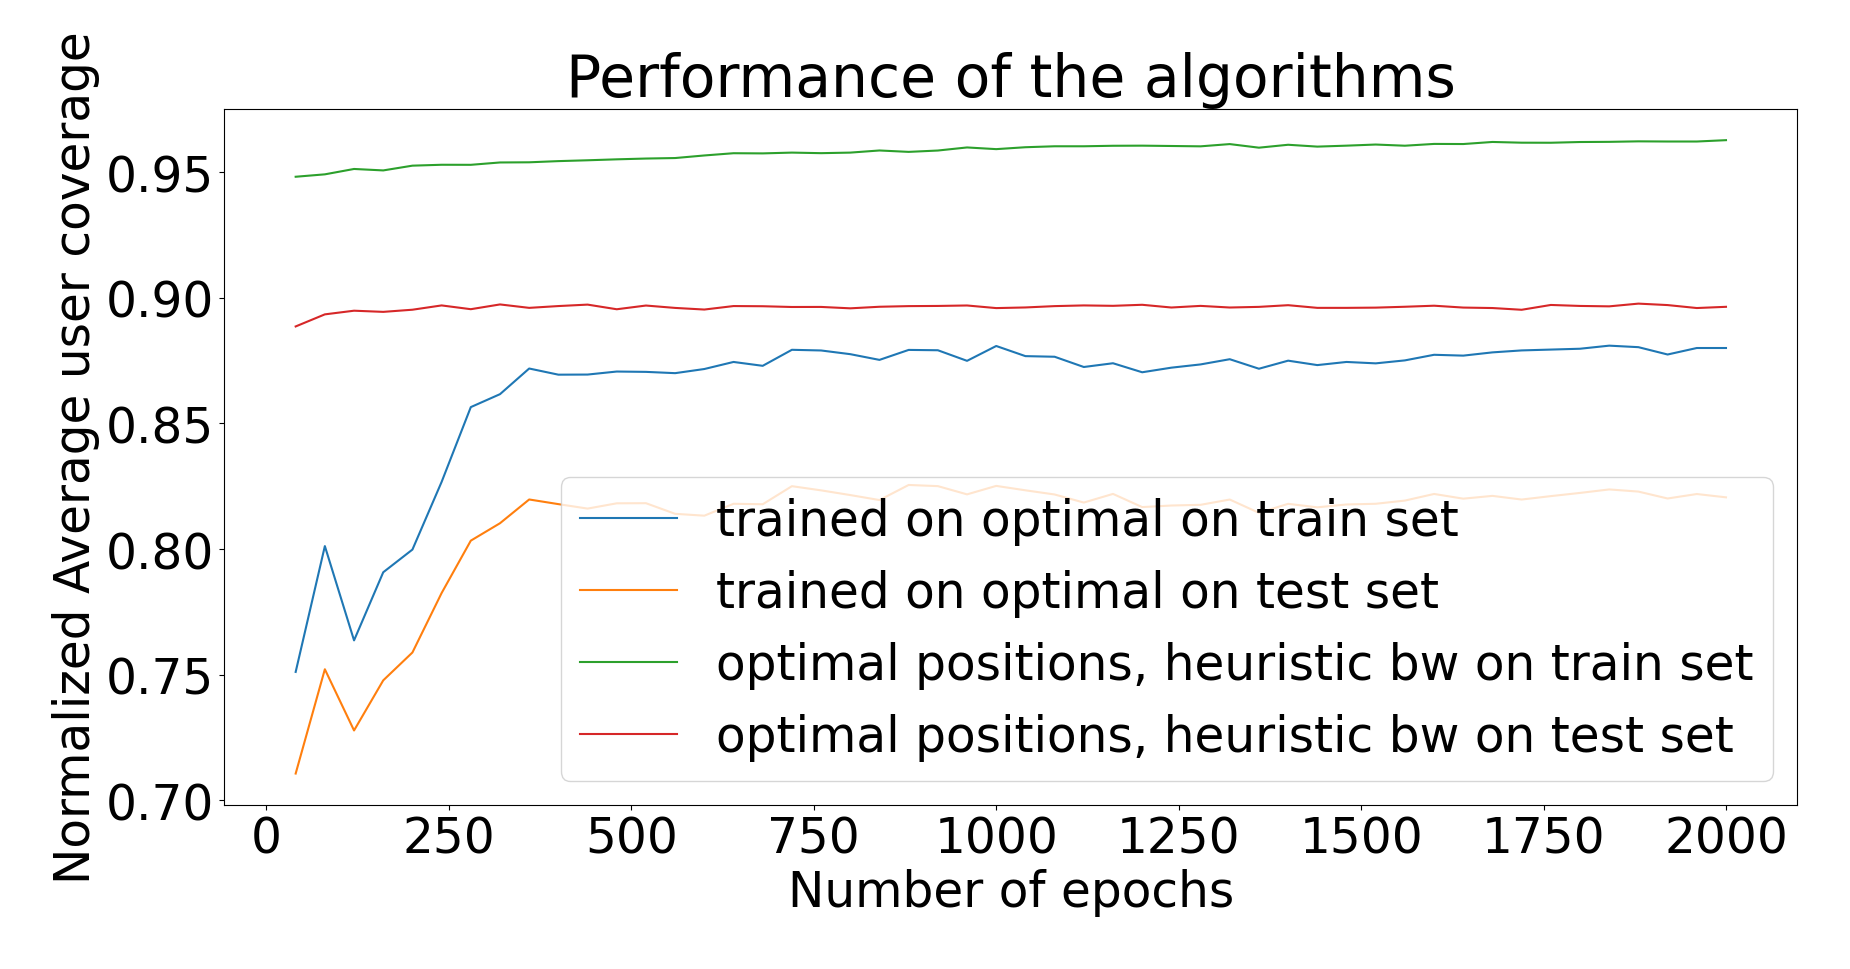
\includegraphics[width=0.5\textwidth]{images/bilan_en _fonction epochs_aibw.png}
    \caption{Performance with optimal positions and AI bandwiths}
\end{figure}

As we can see, the bandwidth part seems to be the issue.

Thus, I implemented an agent which decides positions with a neural network, but decides the bandwiths optimally,
which is pretty fast once the positions are fixed.

We then have the following results:

\begin{figure}[H]
    \centering
    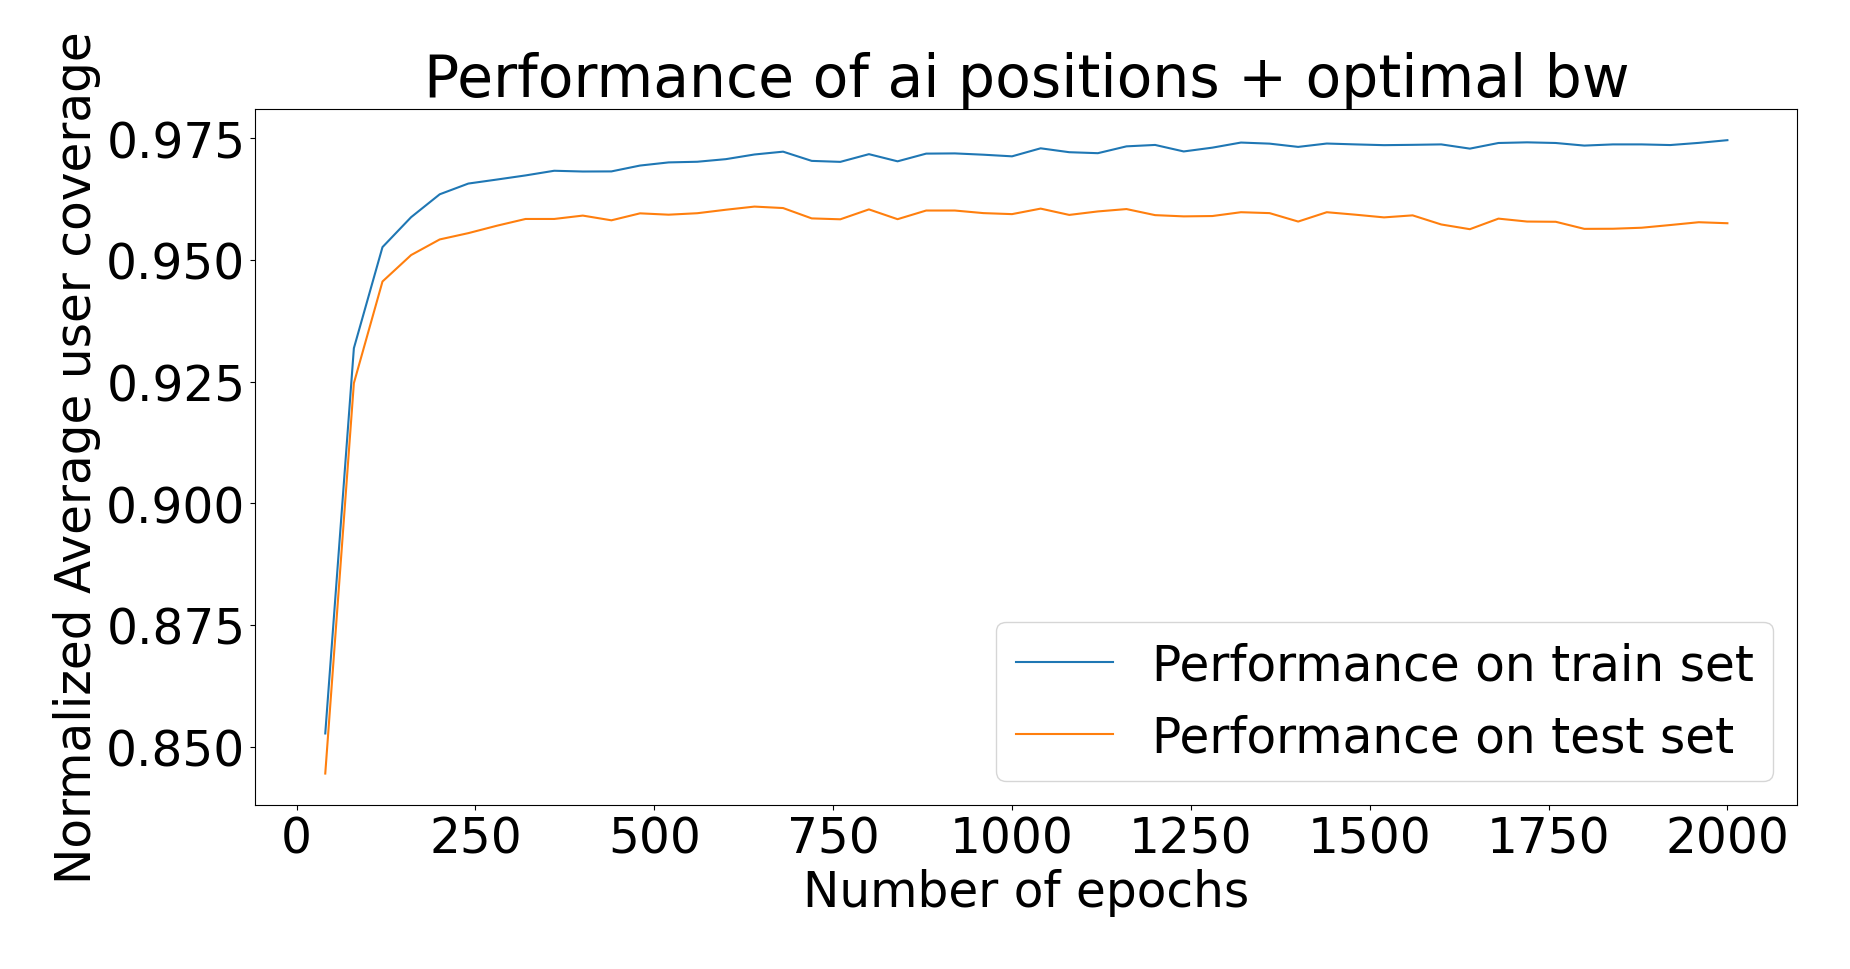
\includegraphics[width=0.5\textwidth]{images/mix_results.png}
    \caption{Performance with AI positions and optimal bandwiths}
\end{figure}

To do a complete comparaison of the different methods, I computed the mean rewards and time to execute of the 3 methods quoted until now:

\begin{center}
    \begin{tabular}{ c c c }
     Type of agent & Average user coverage & Execution time \\ 
     AI positions and bandwiths & 76.80\% & 0.7875 ms \\  
     AI positions and optimal bandwiths & 84.72\% & 15.677 ms  \\
     Optimal positions and bandwiths &  87.08\% & 2.2759 s 
    \end{tabular}
    \end{center}

\subsection{Generalizing to a variable number of users}

However, until now, I have only resolved instances with a fix number of users.

To fix this, the first solution we imagined was to use graph neural networks.
\textit{Detail how gnn work}

The graph given to the neural network was constructed using a k-neighbourg algorithm.
I have made a graphic plotting the final test error in function of the k in the k-neighbourg algorithm.

However, as you can see, whatever the chosen k is, the results are always lacking.

I thus opted for a simpler but less beautiful approach: I just add a one-hot to each user stating if the drone exists or not.
Thus, the neural network can be used to resolve instances with a variable number of users, as long as the number in question is inferior to a certain maximum.

The precision is very similar to what it used to be with a fix number of users as you can see in the following graphics:

\textit{Put some graphics here}

\section{Ouverture: Utiliser la distance à l'optimum comme erreur pour l'apprentissage}

\section{Conclusion}


\end{document}


